\documentclass{llncs}

\usepackage{url}
\usepackage{amsmath}
\usepackage{amssymb}
\usepackage{zed-cm}
\usepackage{booktabs}
\usepackage{color}
\usepackage{alltt}
\usepackage{boxedminipage}
\usepackage{graphicx}

\title{PODD -- An End-to-end Semantic Data Management System}

\author{Yuan-Fang Li$^\dagger$, Gavin Kennedy$^{\S,\sharp}$, Faith Ngoran$^\S$, Philip Wu$^\P$, Jane Hunter$^\S$}

\institute{
$^\dagger$Clayton School of IT, Monash University\\
$^\S$School of ITEE, The University of Queensland\\
$^\sharp$High Resolution Plant Phenomics Centre, Canberra\\
$^\P$The John Curtin School of Medical Research, Australian National University%\\
%Contact: \email{\texttt{yuanfang.li@monash.edu}}
}

\begin{document}
\maketitle

\begin{abstract}
The massive amounts of data and the rapid evolution of data models contribute to making scientific data management a very challenging task. In this paper we present PODD, an ontology-based data management system. In PODD, ontologies are used to completely capture the definition and relationship of domain concepts and object. The open and semantic nature of ontologies makes PODD extensible and amenable for integration and reuse.
\end{abstract}

\section{Introduction}\label{sec:intro}
Data management has become an indispensable part of modern scientific research~\cite{1107503}. Among other factors, there are three core challenges for the effective data management in scientific research. (1) The ability to provide a data management system (DMS) that can manage large quantities of heterogeneous data. (2) The ability to support metadata-related services to provide context and structure for data within the DMS to facilitate effective search, query and dissemination. (3) The ability to accommodate evolving and emerging knowledge, technologies and processes.

Database-based DMS have traditionally been applied successfully to manage
research data. In such approaches, usually the domain model needs to stay relatively stable as database extension and migration is
often an error-prone and laborious task. Consequently, this approach is
not suitable for domains where data and model evolution is the norm
rather than the exception.

Ontology language OWL is both open and semantically precise. It has been successfully used widely a number of domains for knowledge representation and data integration~\cite{journals/bib/RuttenbergRSM09}. In this paper, we present our work in designing PODD (Phenomics Ontology Driven Data Management)~\cite{Li2011}, a semantic, domain-independent DMS system that takes advantage of the intrinsic characteristics of OWL. The
ontology-based domain model is at the core of PODD as it defines the
logical hierarchy of data in scientific experiments.
Data integrity is therefore maintained via ontology reasoning.

\section{The PODD System Achitecture \& Main Functionality}\label{sec:arch}
A most distinguishing characteristic of PODD is its flexibility, which is exhibited in two ways. \emph{Firstly}, the system can be readily applied to another domain with just a change of the underlying domain model (ontologies). \emph{Secondly}, existing concepts and objects can evolve independently without affecting the definition or integrity of each other. 

Such flexibility is achieved by defining domain entities using OWL ontologies, in which: (1)
OWL classes represent domain concepts; (2) OWL properties model concept
attributes and their relationships; (3) OWL restrictions specify
constraints on concepts; (4) OWL individuals define concrete
domain objects where attributes and relationships are defined using OWL
assertions, and finally (5) OWL annotations express auxiliary information. Raw data files are attached to concrete domain objects.

\vspace{-12pt}
\begin{figure}[htb]
\centering
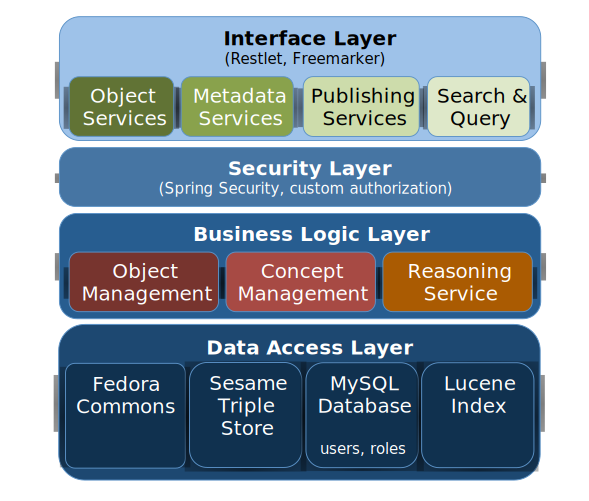
\includegraphics[trim = 64mm 15mm 52mm 28mm, clip,width=64mm]{podd_arch.pdf}
\vspace{-16pt} \caption{The high-level architecture and components in PODD.}\label{fig:arch}
\end{figure}

\vspace{-8pt}
The high-level design of PODD takes a modular and layered approach, as can be seen in Figure~\ref{fig:arch}. The foundation \textbf{data access layer} is responsible for low-level tasks (creation, modification and deletion of concepts and objects), consisting of an underlying repository system (Fedora Commons), an RDF triple store (OpenRDF Sesame), an in-house database
that stores essential information and a full-text search engine (Apache Lucene). The \textbf{business logic layer} in the middle is responsible for managing
concepts and objects, such as versioning, object conversion and
integrity validation. The \textbf{security layer} controls access
(authentication and authorization) to concepts and objects and guards
all operations on them. Secure channels (HTTPS) and Shibboleth\footnote{\url{http://shibboleth.internet2.edu/}} integration have also beeb developed for more secure and flexible access to the system.
At the top of the stack is the \textbf{interface layer}, where the data
management system can be accessed using a number of interfaces such as
a Web browser or API calls. 

Data can be deposited in PODD through the Web interface and Web Services. Information stored in PODD can be retrieved in a number of ways: (1) manual browsing (shown in Figure~\ref{fig:browser}), (2) SPARQL queries, (3) Lucene full-text search, (4) Web Services through REST-style APIs and (5) automated harvesting through RDFa and OAI-PMH annotations.

\section{Ontology-based Domain Modeling}\label{sec:ont}
In our modeling approach, ontologies are developed on multiple levels. The base ontology defines domain-independent concepts and their inter-relationships with each other. Based on this ontology, other more domain-specific ontologies are developed hierarchically. To describe knowledge in phenomics, for example, we extend the base ontology
by defining additional concepts including \emph{Genotype}, \emph{Gene},
\emph{Phenotype} and \emph{Sequence} as subclasses of
existing ones. Additional OWL object and datatype properties are
also defined to model the attributes and relationships of these
concepts, as shown in Figure~\ref{fig:podd_high}. These ontologies play a vital role in all major data management life cycles, including ingestion, retrieval, update and publication.

\vspace{-20pt}
\begin{figure}[htb]
\centering
\includegraphics[trim = 2mm 0mm 2mm 0mm, clip,width=\textwidth]{ont_podd.pdf}
\vspace{-16pt} \caption{Extended Domain Ontology for
phenomics.}\label{fig:podd_high}
\end{figure}

\vspace{-32pt}
\section{PODD Deployment}\label{sec:podd}
PODD has been successfully deployed at two different Australian research institutes to satisfy their data management needs. An instance of PODD has been deployed in production for the Australian Plant Phenomics Facility (APPF)\footnote{\url{http://podd.plantphenomics.org.au/}}. Another instance has been deployed in production for the Australian Phenomics Network (APN)\footnote{\url{http://podd.australianphenomics.org.au/}} for mouse phenomics research. The source code of the PODD repository software has been published in this repository\footnote{\url{http://podd.plantphenomics.org.au/podd/object/poddObject:696}}. Such deployments demonstrates the versatility of the system.

\vspace{-8pt}
\begin{figure}[htb]
\centering
\includegraphics[trim = 5mm 0mm 5mm 0mm, clip,width=\textwidth]{browser.png}
\vspace{-8pt} \caption{The browser view of a plant project in a PODD
DMS.}\label{fig:browser}
\end{figure}

%\vspace{-24pt}
\section{Conclusion}\label{sec:concl}
In this demonstration, we present the PODD data management system. Modelling domain entities entirely in OWL ontologies, PODD takes advantage of the intrinsic semantic rigor and openness of the OWL language. Therefore, PODD is characterized by great flexibility and extensibility. It is also amenable to semantic integration and interoperability.

\section*{Acknowledgment}
This work is part of a National eResearch Architecture Taskforce (NeAT) project, supported by the Australian National Data Service (ANDS) through the Education Investment Fund (EIF) Super Science Initiative, and the Australian Research Collaboration Service (ARCS) through the National Collaborative Research Infrastructure Strategy Program. 

\bibliography{all,liyf}
\bibliographystyle{abbrv}
\end{document}
